
% --------------------------------------------------------------
\begin{frame}[fragile]
  \frametitle{Coupling : Explicit Method Stability}
  \begin{figure}[htbp!]
    \begin{center}
      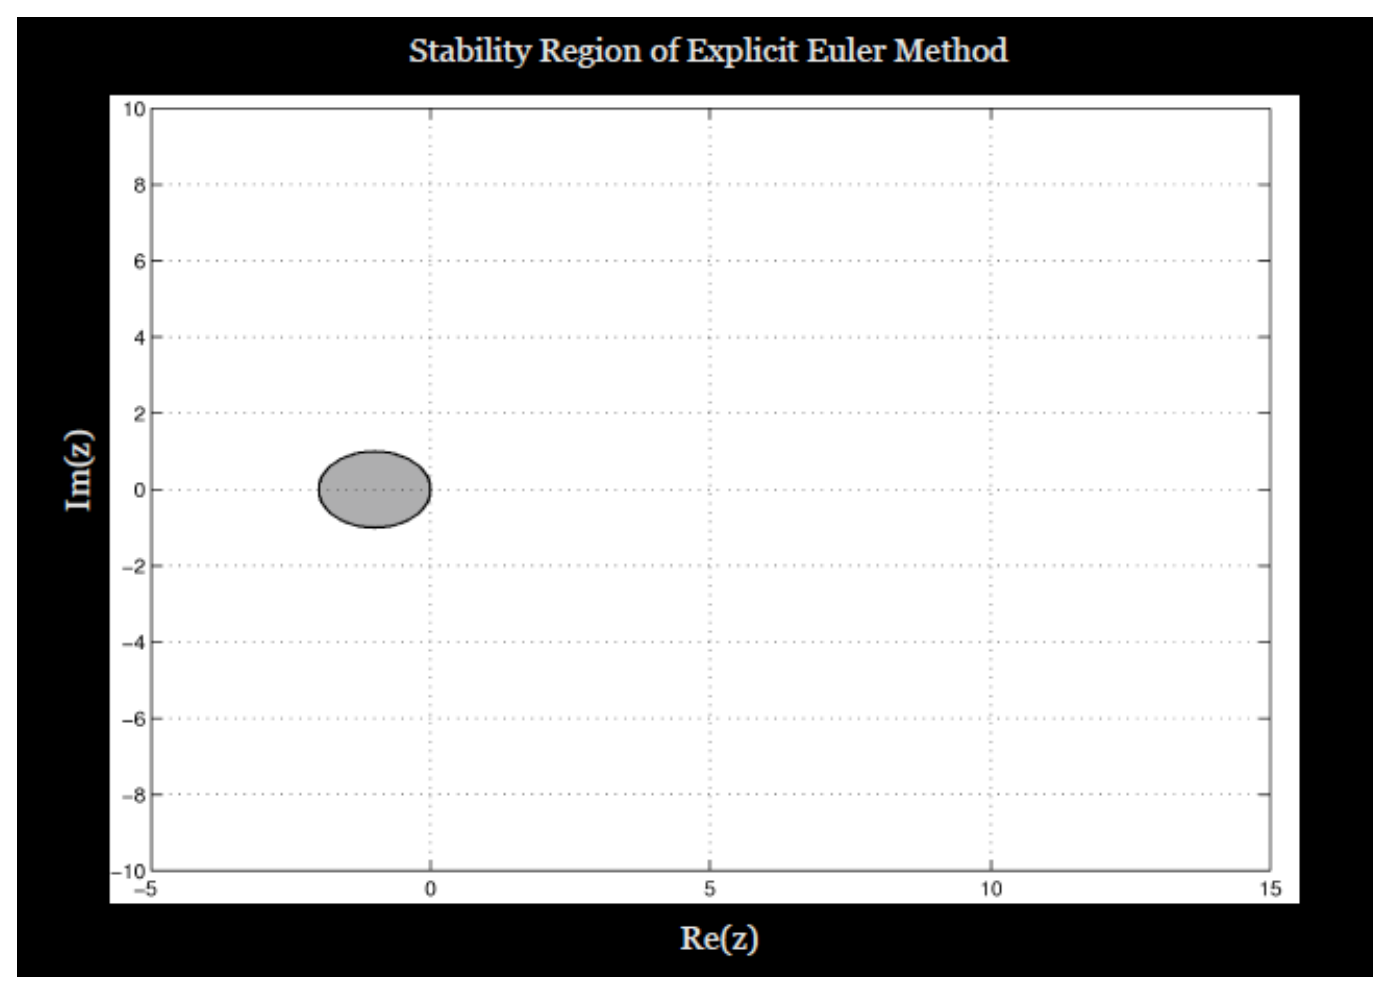
\includegraphics[width=0.8\textwidth]{./progress/euler.eps}
    \end{center}
    \caption{In addition to the loss of nonlinear residuals in the operator 
    splitting technique, the small stability region of explicit Runge-Kutta methods is 
  a drawback.}
    \label{fig:euler_stability}
  \end{figure}

\end{frame}

% --------------------------------------------------------------
\begin{frame}[fragile]
  \frametitle{Coupling : Implicit Method Stability}
  \begin{figure}[htbp!]
    \begin{center}
      \includegraphics[width=0.8\textwidth]{./progress/radau.eps}
    \end{center}
    \caption{Implicit Runge-Kutta methods, however, can be more stable. RadauII-5, for example, has a large stability region.}
    \label{fig:radau_stability}
  \end{figure}

\end{frame}


% --------------------------------------------------------------
\begin{frame}[fragile]
  \frametitle{Coupling : Jacobian}
BUT, recasting the whole problem into a Newton's solve for implicit Runge-Kutta
requires calculation of the Jacobian matrix. Direct computation of the (22x22)
Jacobian is overly complex. 
\end{frame}

% --------------------------------------------------------------
\begin{frame}[fragile]
  \frametitle{Coupling : Jacobian Free Newton Krylov}
However, Jacobian Free Newton-Krylov solves this issue. Thus, an implicit JFNK 
framework should be used to construct the more complex, 3D simulations. 

\end{frame}

% --------------------------------------------------------------
\begin{frame}[fragile]
  \frametitle{Coupling : Tools Available}
  \begin{figure}[htbp!]
    \begin{center}
      \includegraphics[height=0.7\textheight]{./progress/pronghorn_bench.eps}
    \end{center}
    \caption{PBMR-400 Benchmark}
    \label{fig:pbmr400}
  \end{figure}
\end{frame}

% --------------------------------------------------------------
\begin{frame}[fragile]
  \frametitle{Coupling : Potential Future Work}
    \begin{itemize}
    \item 3D Steady State Neutronics, Fixed Cross Sections 
    \item 3D Steady State Thermal Hydraulics, Fixed Power, Compare to COMSOL 
    \item Coupled 3D Steady State N\&TH
    \item Transients - LOFC, LOHS, LOLA, RIA
    \item Startup Modeling
    \item Randomly Packed Bed Analyses
    \item Xenon Stability
    \end{itemize}
\end{frame}

% --------------------------------------------------------------
\begin{frame}[fragile]
  \frametitle{Coupling : MOOSE}
  One of the first steps to using MOOSE is building a mesh. 
  See github.com/katyhuff/pbfhr .

  \begin{figure}[htbp!]
    \begin{center}
      \includegraphics[height=0.6\textheight]{./progress/bunny.eps}
    \end{center}
    \caption{A mesh is a computational data object that holds nodes, edges, and 
    attributes}
    \label{fig:radau_stability}
  \end{figure}

\end{frame}

